\documentclass[oneside, 12pt]{book}

% ------------------------------------------------------------------------------
% Setup for table of contents
\setcounter{tocdepth}{3} 	% TOC should label down to subsubsections
\setcounter{secnumdepth}{2}	% TOC should not number further than a subsection number
% ------------------------------------------------------------------------------


% ------------------------------------------------------------------------------
% General Setup
\usepackage[english]{babel}
\usepackage{amsfonts, amsmath, amsthm}		% Formatting symbols, theorems, lemmas, definitions, and examples

\usepackage{float}							% For making sure tables and figures stay in place
\usepackage{fullpage}						% Create ~1" margins
\usepackage[bottom,flushmargin]{footmisc}	% Put footnotes at bottom of page; don't intent footnotes
\usepackage[titletoc]{appendix}

\setcounter{chapter}{-1}				% Start with chapter 0

\usepackage{enumitem}					% For custom labels on enumerations
\usepackage{hyperref}					% For inserting links
\usepackage{graphicx} 					% For inserting images

% Tikz stuff
\usepackage{tikz}
\usetikzlibrary{patterns}
\usetikzlibrary{calc,patterns,decorations.pathmorphing,decorations.markings}
% ------------------------------------------------------------------------------

% ------------------------------------------------------------------------------
% Theorems, lemmas, definitions and examples should not be numbered
\newtheorem*{theorem}{Theorem}
\newtheorem*{definition}{Definition}
\newtheorem*{lemma}{Lemma}
\newtheorem*{example}{Example}
% ------------------------------------------------------------------------------

% ------------------------------------------------------------------------------
% Shortcuts
\newcommand{\dd}[2]{\frac{\mathrm{d} #1}{\mathrm{d} #2}}							% d[] / d[]

\newcommand{\abs}[1]{\lvert #1 \rvert}												% absolute value

\DeclareMathOperator{\arcsec}{arcsec}												% arc-secant
\DeclareMathOperator{\arccot}{arccot}												% arc-cotangent
\DeclareMathOperator{\arccsc}{arccsc}												% arc-cosecant

\newcommand{\R}{\mathbb{R}}															% Real numbers
% ------------------------------------------------------------------------------

\begin{document}
	% Title page setup
	\title{Single Variable Calculus: A Summary}
	\author{William Boyles}
	\date{}
	
	\frontmatter
		\maketitle
		\tableofcontents
		
	\mainmatter
		\chapter{Background \& Review}
Everything mentioned in this chapter should already be familiar to you from other math classes.
These topics span two major areas: algebra/pre-calculus and limits.
Ideas from these topics will often be used implicitly or without a passing reference. \\

If you are unfamiliar with anything mentioned, you can use many of the great online resources like Khan Academy to familiarize yourself before moving forward.

\section{Algebra and Pre-Calculus}
\noindent

\subsection{Sets}
\begin{definition}
	A set $A$ is a collection of distinct elements. Those elements can be anything, like numbers, functions, and even other sets.
\end{definition}
We can define a set by giving its elements, like $A = \{-2, 5, 3\}$ or by describing its properties, like $A = \{x \mid x > 0\}$ where the vertical bar means "such that".
If an object $x$ is a member of the set $A$, we write $x\in A$.\bigskip


\noindent
A set $A$ is called a subset of a set $B$ if every element of $A$ is also an element of $B$. 
We can write this as $A \subseteq B$. 
For example, $\{7, 10, 16\} \subseteq \{5, 6, 7, 9, 10, 11, 16\}$. 
Note that this relation can be strict if there exists at least one element in $B$ that is not also an element of $A$. 
Some common sets and their informal definitions are given below:

\begin{table}[H]
	\centering
	\begin{tabular}{c|c|c}
		Set Name & Symbol & Informal Definition                                                                                                                         \\ \hline
		Natural numbers & $\mathbb{N}$ & $\{1, 2, 3, \dots\}$           						                                                                        \\
		Integers & $\mathbb{Z}$ & $\{\dots, -3, -2, -1, 0, 1, 2, 3, \dots\}$                                                                                            \\
		Rational numbers & $\mathbb{Q}$ & $\{\frac{m}{n} \mid m,n \in\mathbb{Z}$ and $n \neq 0\}$                                                                       \\
		Real numbers & $\mathbb{R}$ & Any number on the number line\footnote{Sadly, there is no way to give a stronger formal definition without higher mathematics.}   \\
	\end{tabular}
\end{table}

This means that $\mathbb{N} \subset \mathbb{Z} \subset \mathbb{Q} \subset \mathbb{R}$.\bigskip


\noindent
There are several common operations that can be performed on sets.
The union $A \cup B$ of two sets $A$ and $B$ is the set of all elements that are elements of $A$ or of $B$. 
Similarly, the intersection $A \cap B$ of two sets $A$ and $B$ is the set of all elements that are also elements of both $A$ and $B$.
\begin{example}
	If $A = \{\sqrt{2}, 2, 5, 8\}$ and $B = \{-9, 8, 2.3\}$, what are $A \cup B$ and $A \cap B$?		
\end{example}
To find the union, we combine the sets, making sure to include any repeated element only once:
\begin{equation*}
	A \cup B = \{-9, \sqrt{2}, 2, 2.3, 5, 8\}.
\end{equation*}
Then, since the only element both sets share is 8, we also have
\begin{equation*}
	A \cap B = \{8\}.
\end{equation*}

\subsection{Intervals}
\begin{definition}
	We call a subset $I$ of $\mathbb{R}$ an interval if, for any $a, b \in I$ and $x \in \mathbb{R}$ such that $a \leq x \leq b$, then $x \in I$. 
\end{definition}
We can write an interval more simply using the notation $[a, b]$, which is equivalent to $\{x \in \mathbb{R} \mid a \leq x \leq b\}$. 
This is called a closed interval, and to make the inequalities strict, we can also define an open interval by using parantheses instead of square brackets.\bigskip

In addition, we can mix the two to create half-open intervals, where one inequality is strict and the other isn't. 
For instance, $(2, 5]$ refers to the set $\{x \in \mathbb{R} \mid x < 2 \leq 5\}$
Finally, if the interval is unbounded in either direction, we use the notations $-\infty$ and $\infty$ to indicate that there is no minimum or maximum, respectively.

\begin{example}
	Is $8 \in (-\infty, 4) \cup [8, 100)$?
\end{example}
\begin{answer}
	Since $8 \leq 8 < 100$ is a true statement, $8 \in [8, 100)$. 
	Since we are taking the union with another set, all of the members of the right interval will also be members of the union of intervals. 
	Therefore, the statement is true.
\end{answer}                       % Sets
\subsection{Functions}
\begin{definition}
    A function $f$ is a rule between a pair of sets, denoted $f: D \to C$, that assigns values from the first set, the domain $D$, to the second set, the codomain $C$.
\end{definition}

We call the subset of the codomain $C$ that constitutes all values $f$ can actually attain the range $R \subseteq C$. 
Note that when we draw a graph of a function, all we are doing is drawing all ordered pairs $\{(x, f(x)) \mid x \in D\}$.

\begin{example}
    Find the domain of the following function:
    \begin{equation*}
        f(x) = \frac{1}{(1 - x)\sqrt{5 - x^2}}
    \end{equation*}
\end{example}

\begin{answer}
    We know that $\frac{n}{0}$ is undefined for all $n \in \mathbb{R}$ and $\sqrt{x}$ is only defined for $x \geq 0$. 
    The first condition applies to the first term in the denominator and both conditions apply to the second, giving us
    \begin{equation*}
        (1 - x) \neq 0 \text{ and } 5 - x^2 > 0
    \end{equation*}
    The first condition implies $x \neq 1$ while the second implies $|x| < \sqrt{5}$.
    Putting these together, we find that the domain is
    \begin{equation*}
        \{x \mid x \neq 1, |x| < \sqrt{5}\} \text{ or } (-\sqrt{5}, 1) \cup (1, \sqrt{5})
    \end{equation*}
\end{answer}

We can also compose two functions, such that the ouput of one function is the input of another: 
\begin{equation*}
    (f \circ g)(x) = f(g(x)).
\end{equation*}

\begin{definition}
    A function $g$ is called an inverse function of $f$ if $f(g(x)) = x$ for all x in the domain of g and $g(f(x))$ for all x in the domain of f. 
    We write this as $g = f^{-1}$.
\end{definition}

One common algorithm for finding an inverse function is to set $y = f(x)$, substitute all $x$'s for $y$'s, and then solve for y.
\begin{example}
    Find the inverse function of 
    \begin{equation*}
        f(x) = \frac{5x + 2}{4x - 3}.
    \end{equation*}
\end{example}
\begin{answer}
    We first make the substitutions to set up the algorithm:
    \begin{equation*}
        y = \frac{5x + 2}{4x - 3} \text{ followed by }
        x = \frac{5y + 2}{4y - 3}
    \end{equation*}
    After multiplying both sides by the denominator and simplifying, we have
    \begin{equation*}
        \implies 4xy - 3x = -5y - 2 \\
        \implies y = f^{-1}(x) = \frac{3x - 2}{4x + 5}.
    \end{equation*}
\end{answer}

We say that a function $f$ is even if it satisfies $f(-x) = f(x)$ for all $x \in D$.
Likewise, we say that a function $f$ is odd if it satisfies $f(-x) = -f(x)$ for all $x \in D$. 
Geometrically, we can see that the graph of an even function is symmetric with respect to the $y$-axis, while the graph of an odd function is symmetric with respect to the origin. 

\begin{example}
    Is $f(x) = 2x - x^2$ even, odd, or neither?
\end{example}
\begin{answer}
    \begin{equation*}
        f(-x) = 2(-x) - (-x)^2 = -2x - x^2
    \end{equation*}
    Since $f(-x) \neq f(x)$ and $f(-x) \neq -f(x)$, the function is neither even nor odd.
\end{answer}                   % Functions
\subsection{Complex Numbers}
\begin{definition}
	$i$ is called the imaginary unit. It's defined by $i^2 = -1$.
\end{definition}


\noindent
Complex numbers ($\mathbb{C}$) have the form $z = \alpha + \beta i$, where $\alpha$ and $\beta$ are real numbers. The $\alpha$ part of $z$ is called the real part, so $\Re(z) = \alpha$. The $\beta$ part of $z$ is called the imaginary part, so $\Im(z) = \beta i$.\\

\noindent
Often, complex numbers are visualized as points or vectors in a 2D plane, called the complex plane, where $\alpha$ is the x-component, and $\beta$ is the y-component. Thinking of complex numbers like points helps us define the magnitude of complex numbers and compare them. Since a point $(x,y)$ has a distance $\sqrt{x^2+y^2}$ from the origin, we can say the magnitude of $z$, $\lvert z \rvert$ is $\sqrt{\alpha^2 + \beta^2}$. Thinking of complex numbers like vectors helps us understand adding two complex numbers, since you just add the components like vectors.\\

\noindent
A common operation on complex numbers is the complex conjugate. The complex conjugate of $z = \alpha + \beta i$ is $\overline{z} = \alpha - \beta i$. $z$ and $\overline{z}$ are called a conjugate pair.\\

\noindent
Conjugate pairs have the following properties.
Let $z, w \in \mathbb{C}$.
\begin{align*}
	\overline{z \pm w} &= \overline{z} \pm \overline{w} \\
	\overline{zw} &= \overline{z}\overline{w} \\
	\overline{z} &= z \Leftrightarrow z \in \mathbb{R} \\
	z\overline{z} &= \lvert z \rvert^2 = \lvert \overline{z} \rvert^2 \\
	\overline{\overline{z}} &= z \\
	\overline{z}^n &= \overline{z^n} \\
	z^{-1} &= \frac{\overline{z}}{\lvert z \rvert^2} 
\end{align*}
 			% Complex Numbers
\subsection{Factoring Polynomials}
\noindent
We want to break up a polynomial like $f(x) = a_0 + a_1x^1 + \ldots a_nx^n$ into linear factors so that $f(x) = c(x-b_1)\cdot \ldots \cdot(x - b_n)$. This form makes it simple to see that the roots of $f$, solutions to $f(x) = 0$, are $x = b_1 \ldots b_n$.\\

\noindent
For quadratics, $f(x) = ax^2 + bx + c$, there exists a simple formula that will give us both roots, the quadratic formula
\begin{equation*}
	x = \frac{-b \pm \sqrt{b^2-4ac}}{2a}.
\end{equation*}

\noindent
We can see that when $b^2 - 4ac < 0$, like for $f(x) = x^2 + 5x + 10$, we will get complex roots $\alpha \pm \beta i$. For any polynomial, these roots come in pairs, so if $\alpha + \beta i$ is a root, then so is $\alpha - \beta i$. This means that every conjugate pair $\alpha \pm \beta i$ has a quadratic equation with those roots. Sometimes we will not factor quadratics with complex roots into linear terms.\\

\noindent
Although there do exist explicit formulas for finding roots for cubic (degree 3) and quartic (degree 4) equations, they are too long and not useful enough to memorize. When working by hand, we instead use other tricks to find roots.\\

\noindent
There are a few useful tricks that can help. If the polynomial doesn't have a constant term, then 0 is a root. If all the coefficients sum to 0, then 1 is a root. For certain polynomials with an even number of terms, like all cubics of the form $ax^3 + bx^2 + cax + cb$ we can factor out a term from the first two and last two terms to get $x^2(ax+b)+c(ax+b) = (ax+b)(x^2+c)$. For other polynomials, we might just try guessing and checking values. However, we need a more efficient way that works in general.\\

\noindent
Since we are looking to find linear factors $f(x) = (x-b_1)\cdot \ldots \cdot(x-b_n)$, we can see that the constant term in the polynomial is the product of the roots $b_1 \ldots b_n$. In fact, since the coefficients of polynomials are completely determined by the roots and the leading coefficient, all the coefficients are sums and products of roots. You might remember when factoring quadratics that the coefficient of $x$ term is the sum of the two roots. These rules are called Vieta's formulas.\\

\noindent
So, if we have the constant term, we can check all of its integer factors to see if any are roots. For each root, we can divide, using a technique like synthetic division, to continue finding the rest of the roots. This method is especially useful on tests because the roots tend to be integers.

\input{../common/algebraPreCalc/factoringPolynomials_example.tex} 		% Factoring Polynomials
\subsection{Trig Functions \& The Unit Circle}
\noindent
Imagine aa circle of radius 1 centered at the origin that we'll call the unit circle. The x and y coordinates of a point on the unit circle are completely determined by the angle $\theta$ in radians between the $x$-axis and a line from the origin to the point.\\

\noindent
The function $\cos{\theta}$ tells us x-coordinate of the point, while $\sin{\theta}$ tells us the y-coordinate of the point. The function $\tan{\theta} = \frac{\sin{\theta}}{\cos{\theta}}$ tells us the slope of the line from the origin to the point. Most of the trig functions have geometric interpretations as shown below. The most used ones are $\sin$, $\cos$, $\tan=\frac{\sin}{\cos}$, $\cot = \frac{\cos}{\sin}$, $\csc=\frac{1}{\sin}$, and $\sec=\frac{1}{\cos}$.

\begin{figure}[H]
	\label{unitCircle}
	\centering
	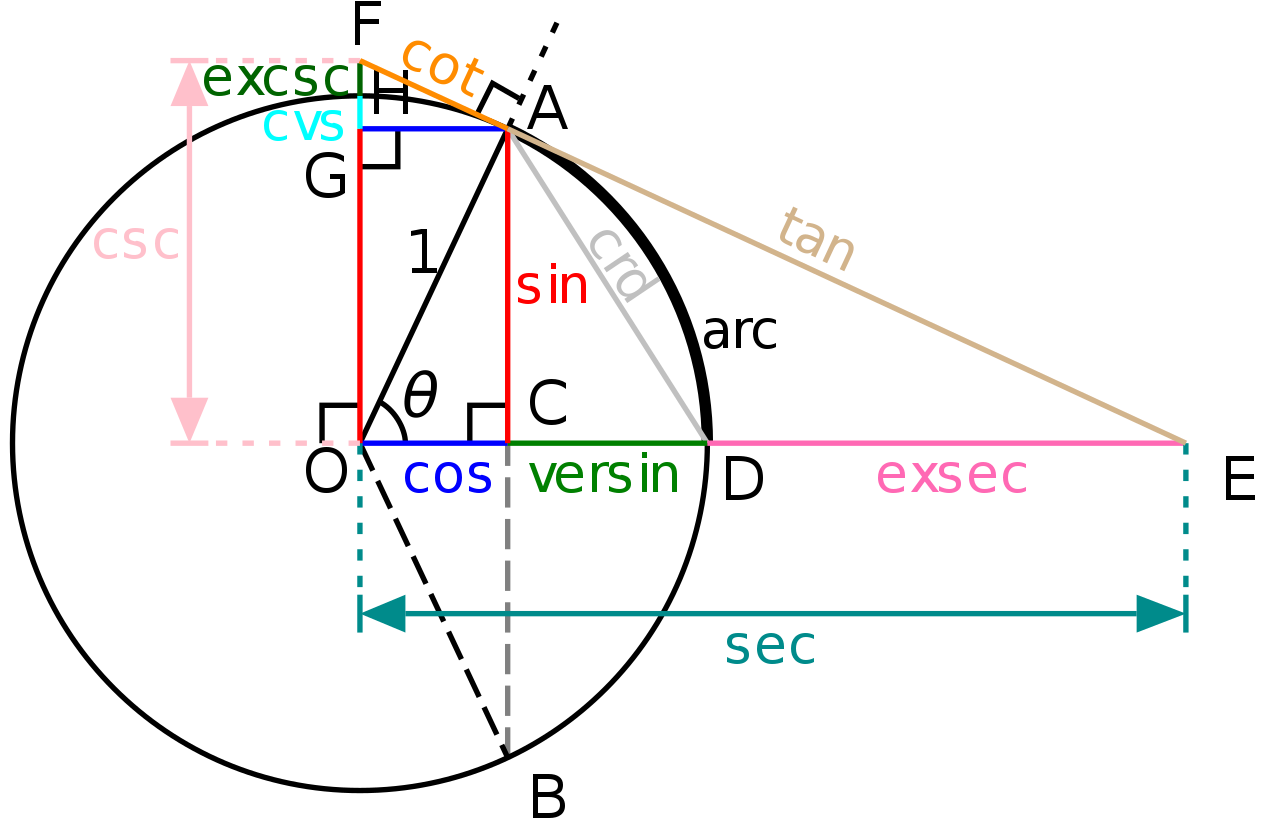
\includegraphics[width = 0.75\textwidth]{../common/algebraPreCalc/unitCircle2.png}
	\caption{\hyperref{https://en.wikipedia.org/wiki/Unit_circle}{}{}{Wikipedia - Unit circle}}
\end{figure}

\noindent
We can also think about the inverses of these trig functions. These are either notated with a -1 exponent on the function, or the prefix arc in front of the function name. Many of these functions are only defined on a part of the domain $\left[0, 2\pi\right]$. Below is a table of the inverse trig functions and their domains.

\begin{table}[H]
	\centering
	\begin{tabular}{l|l}
		Function  & Domain                                                 \\ \hline
		$\arcsin$ & $\left[-1, 1\right]$           						   \\
		$\arccos$ & $\left[-1, 1\right]$                                   \\
		$\arctan$ & $\left(-\infty, \infty\right)$                         \\
		$\arccot$ & $\left(-\infty, \infty\right)$                         \\
		$\arccsc$ & $\left(-\infty, -1\right] \cup \left[1, \infty\right)$ \\
		$\arcsec$ & $\left(-\infty, -1\right] \cup \left[1, \infty\right)$
	\end{tabular}
\end{table}
 	% Trig Functions / Unit Circle
\subsection{Trig Identities}
\noindent
As we could see in Figure \ref{unitCircle}, $\sin$ and $\cos$ form a right triangle with hypotenuse 1. So, using the Pythagorean Theorem,
\begin{equation*}
	\sin^2{\theta} + \cos^2{\theta} = 1.
\end{equation*}
By dividing by $\sin^2$ or $\cos^2$, we can also get
\begin{equation*}
	1 + \cot^2{\theta} = \csc^2{\theta} \text{ and } \tan^2{\theta} + 1 = \sec^2{\theta}.
\end{equation*}
Together, these 3 identities are called the Pythagorean Identities.\\

\noindent
We can also relate functions and co-functions.
\begin{equation*}
	\text{xxx}(\theta) = \text{coxxx}\left(\frac{\pi}{2} - \theta\right).
\end{equation*}

\noindent
Some of the most useful and used identities are the sum and difference.
\begin{align*}
	\sin{\left(\alpha \pm \beta\right)} &= \sin{\alpha}\cos{\beta} \pm \cos{\alpha}\sin{\beta} \\
	\cos{\left(\alpha \pm \beta\right)} &= \cos{\alpha}\cos{\beta} \mp \sin{\alpha}\sin{\beta} \\
	\tan{\left(\alpha \pm \beta\right)} &= \frac{\tan{\alpha} \pm \tan{\beta}}{1 \mp \tan{\alpha}\tan{\beta}} \\
	\sin{\alpha} \pm \sin{\beta} &= 2\sin{\left(\frac{\alpha \pm \beta}{2}\right)}\cos{\left(\frac{\alpha \mp \beta}{2}\right)} \\
	\cos{\alpha} + \cos{\beta} &= 2\cos{\left(\frac{\alpha + \beta}{2}\right)}\cos{\left(\frac{\alpha - \beta}{2}\right)} \\
	\cos{\alpha} - \cos{\beta} &= -2\sin{\left(\frac{\alpha + \beta}{2}\right)}\sin{\left(\frac{\alpha - \beta}{2}\right)} \\
\end{align*} 			    % Trig Identites
\subsection{Exponentials \& Logarithms}
\begin{definition}
	e is the base of the natural logarithm. It's defined by the limit
	\begin{equation*}
		e = \lim\limits_{n\rightarrow\infty}{\left(1+\frac{1}{n}\right)^n}.
	\end{equation*}
\end{definition}
\noindent
$\exp{x} = e^x$ and $\ln{x}$ are inverse functions of each other such that
\begin{equation*}
	e^{\ln{x}} = x \text{ and } \ln{e^x} = x.
\end{equation*}

\noindent
Just like other exponentials, the normal rules for adding, subtracting, and multiplying exponents apply:
\begin{equation*}
	e^xe^y = e^{x+y} \text{, } \frac{e^x}{e^y}=e^{x-y} \text{, and } \left(e^x\right)^k=e^{xk}.
\end{equation*}

\noindent
Similar rules apply for logarithms:
\begin{equation*}
	\ln{x}+\ln{y} = \ln{xy} \text{, } \ln{x}-\ln{y} = \ln{\left(\frac{x}{y}\right)} \text{, and } \ln{\left(a^b\right)} = b\ln{a}.
\end{equation*}

\noindent
We can also write a logarithm of any base using natural logarithms:
\begin{equation*}
	\log_{b}{a} = \frac{\ln{a}}{\ln{b}}.
\end{equation*}

\noindent
$e$ is also unique in that it is the only real number $a$ satisfying the equation
\begin{equation*}
	\frac{\mathrm{d}}{\mathrm{d}x}a^x = a^x,
\end{equation*}
meaning $e^x$ is its own derivative. 		% Exponential and logarithms
\subsection{Partial Fractions}
\noindent
If we have a function of two polynomials $f(x) = \frac{P(x)}{Q(x)}$, it's often easier to break this quotient into a sum of parts where the denominator is a linear or quadratic factor and the numerator is always a smaller degree than the denominator.

\begin{example}
	\begin{equation*}
		\frac{2x-1}{x^3-6x^2+11x-6} = \frac{1/2}{x-1}+\frac{-3}{x-2}+\frac{5/2}{x-3}.
	\end{equation*}
\end{example}

\noindent
One natural way to find these small denominators comes from the linear factors of the denominator where we keep quadratics with complex roots.
This way, when making a common denominator, we get back the original big denominator.
However, there are a few special cases we have to take care of.

\input{../common/algebraPreCalc/linearFactors.tex}
\input{../common/algebraPreCalc/repeatedLinearFactors.tex}
\input{../common/algebraPreCalc/quadraticFactors.tex}
\input{../common/algebraPreCalc/repeatedQuadraticFactors.tex}
\input{../common/algebraPreCalc/improperFractions.tex}
 			% Partial Fractions % Algebra and Pre-Calc
		\chapter{Limits \& Continuity}

Limits are a way of describing what happens to a function $f(x)$ as $x$ gets arbitrarily close to a value from some direction (positive or negative).
This allows us not only to deal with ``holes'' in some functions but describe some of the building blocks of calculus, namely the derivative.

\section{Limit Definition}
\begin{definition}
	Let $f : D \subseteq \R \to \R$.
	Let $c \in R$ be a limit point (ie $c \in D$ or $c$ is on the boundary of $D$).
	$f$ has a limit $L$ as $x$ approaches $c$ if for any given positive real number $\epsilon$, there is a positive real number $\delta$ such that for all $x \in D$,
	\begin{equation}
		0 < \abs{x-c} < \delta \implies \abs{f(x) - L} < \epsilon.
	\end{equation}
	We write this as
	\begin{equation*}
		\lim_{x \to c}{f(x)} = L.	
	\end{equation*}
\end{definition}

\begin{figure}[H]
	\label{unitCircle}
	\centering
	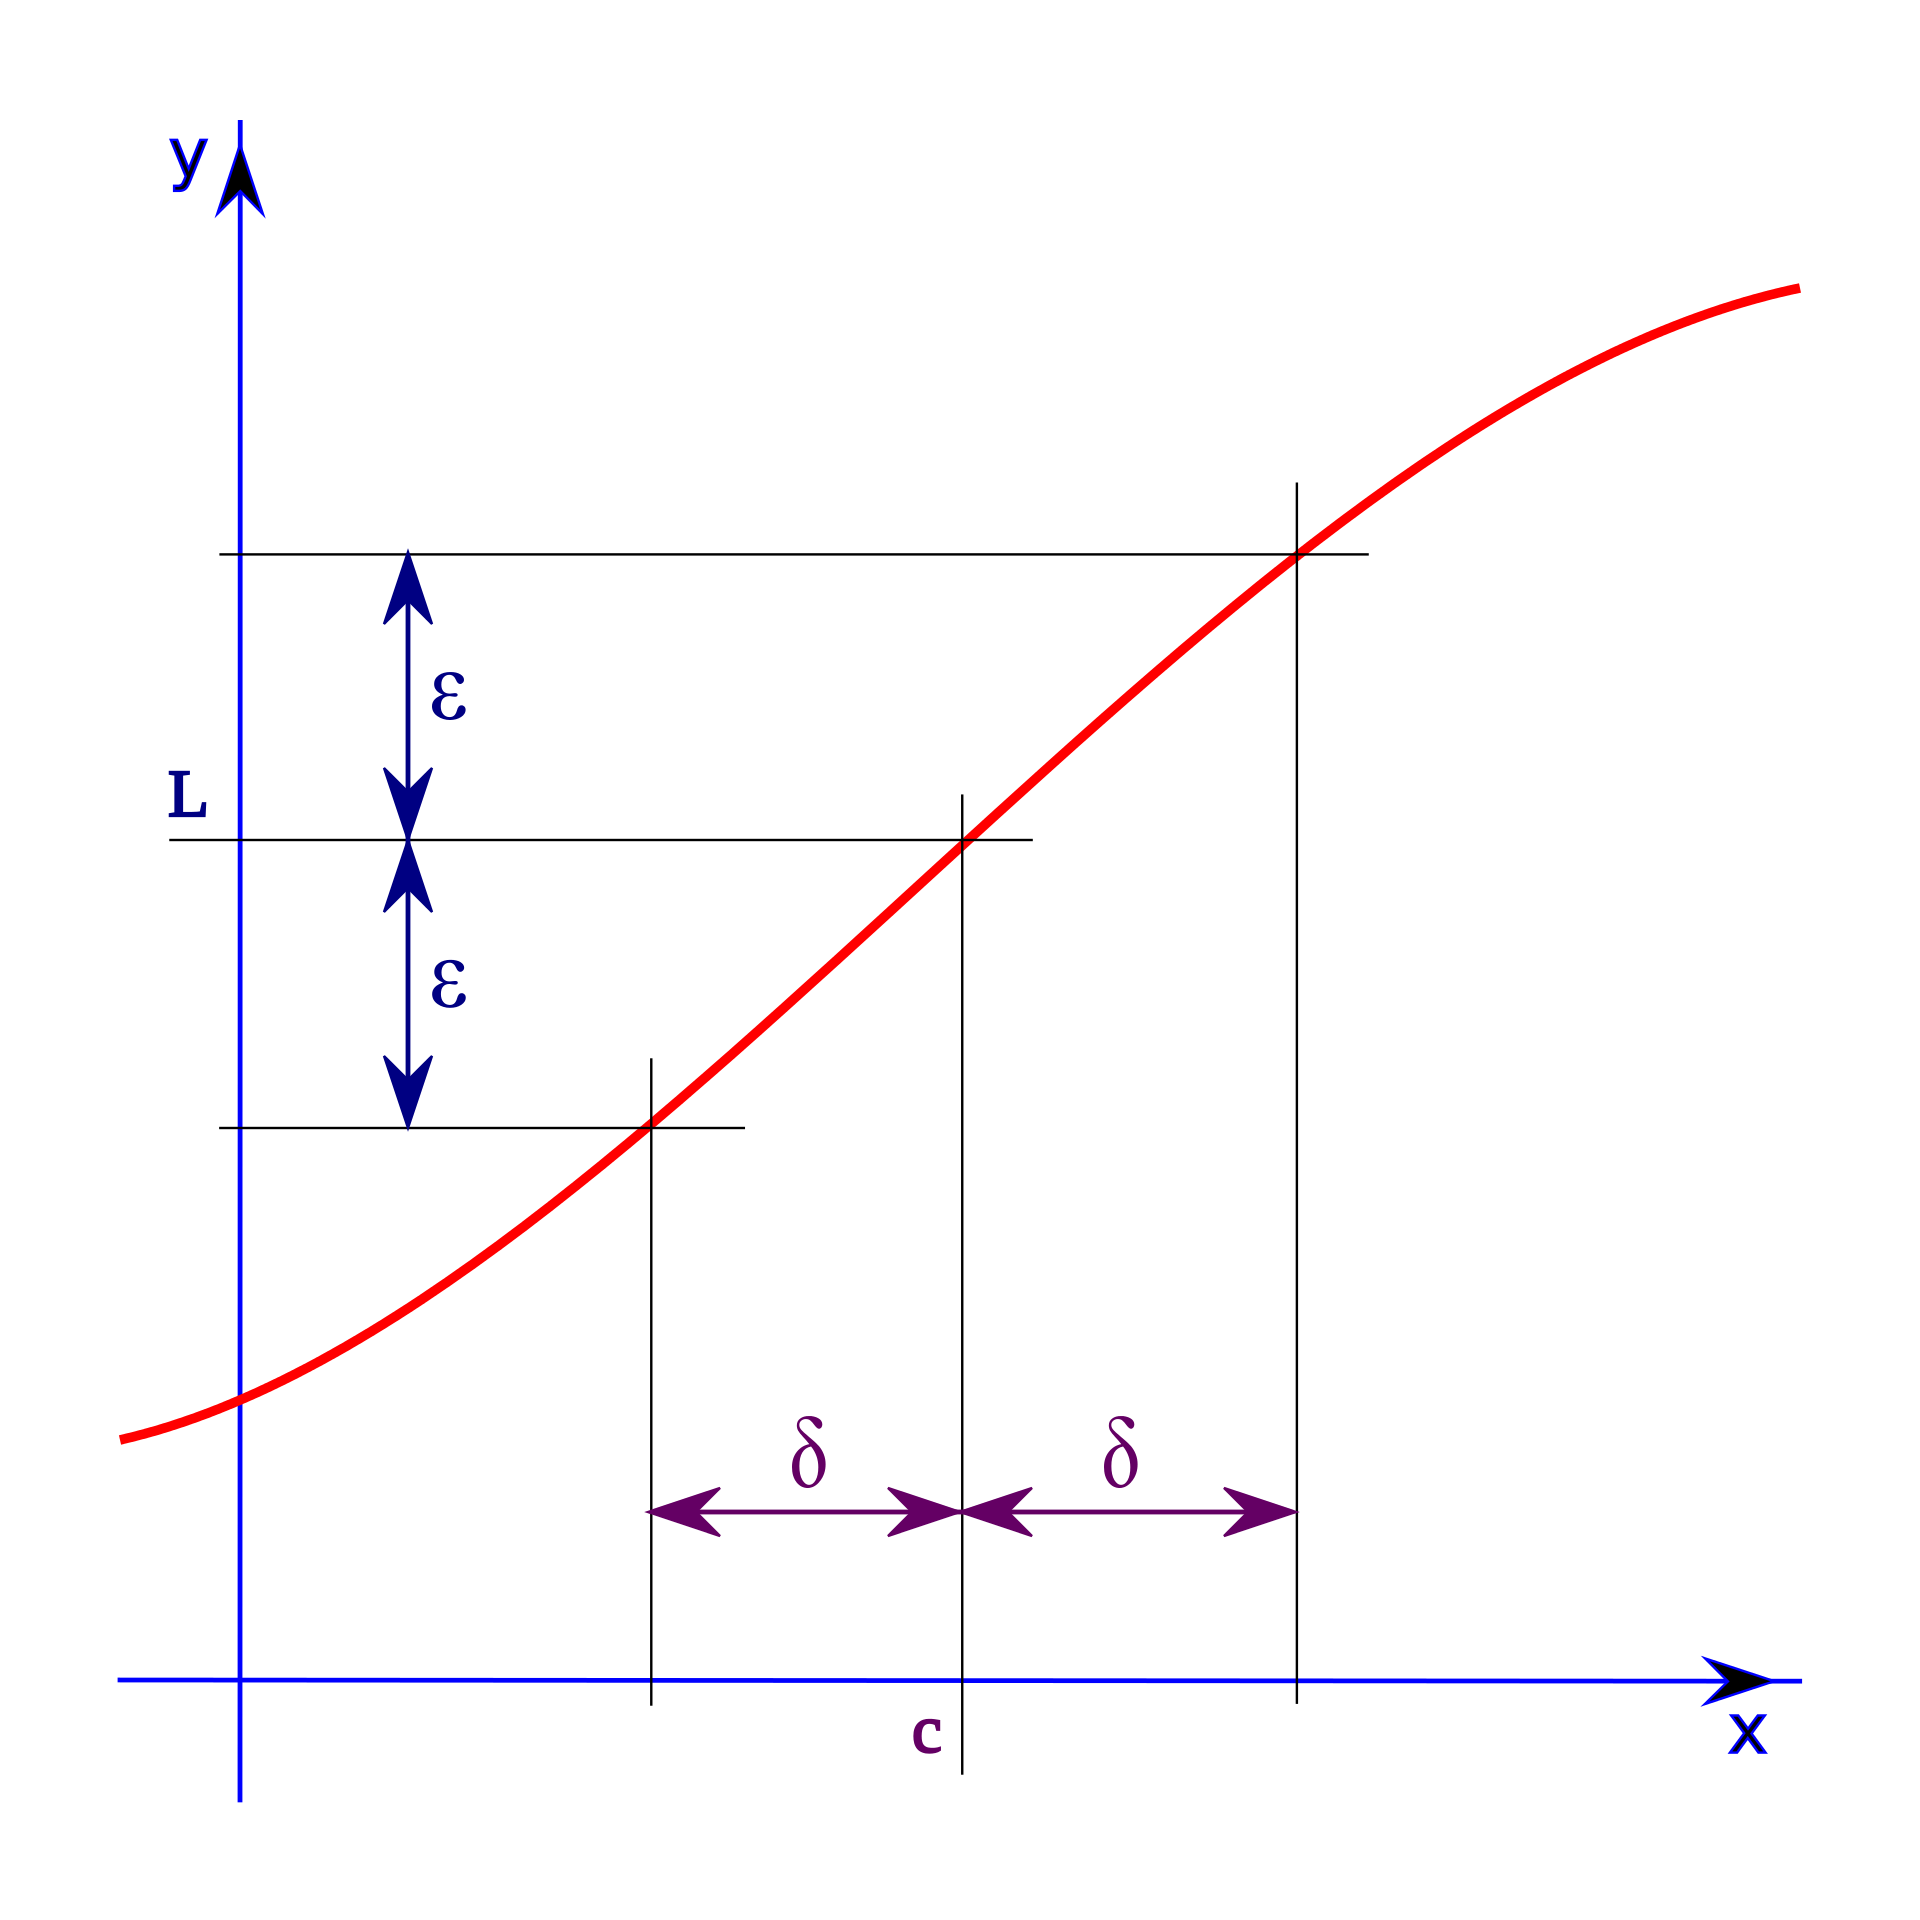
\includegraphics[width = 0.5\textwidth]{./limits_continuity/limit_epsilon_delta.png}
	\caption{\hyperref{https://en.wikipedia.org/wiki/(\%CE\%B5,\_\%CE\%B4)-definition\_of\_limit}{}{}{Wikipedia - $(\epsilon, \delta)\text{-definition of limit}$}}
\end{figure}
\noindent
Visually, what this means is that for any "error bound" of $y$ values $\epsilon$, I can give you a corresponding error bound of $x$ values $\delta$ such that all values of $f(z)$ for $z \in (c -\delta, c+ \delta)$ bound are between $L - \epsilon$ and $L + \epsilon$.

\noindent
We don't use this definition of the limit very often because it's a bit cumbersome.
However, it's important to know that when we use the limit, this is the formal definition making things work.

\begin{example}
	Use the $(\epsilon, \delta)$ definition of the limit to show that
	\begin{equation*}
		\lim_{x\to 0}{x\sin{\frac{1}{x}}} = 0.
	\end{equation*}
\end{example}
Letting $\epsilon > 0$, we need to find corresponding $\delta > 0$ that satisfies the definition for $L = 0$.
Knowing that $\sin$ is bounded between -1 and 1,
\begin{equation*}
	\abs{x\sin{\frac{1}{x}} - 0} = \abs{x\sin{\frac{1}{x}}} = \abs{x}\abs{\sin{\frac{1}{x}}} \leq \abs{x}.
\end{equation*}
\indent
Letting $\delta = \epsilon$, if $0 < \abs{x - 0} < delta$, then $\abs{x\sin{\frac{1}{x}} - 0} \leq \abs{x} < \epsilon$, as required by the definition.
\section{Limit Properties}
Limit have many nice properties all allow us to make useful simplifications when evaluating a limit.
Let
\begin{equation*}
	\lim_{x \to c}{f(x)} = L \text{ and } \lim_{x \to c}{g(x)} = M.
\end{equation*}
\begin{align*}
	\textbf{Sum and Difference Rule: }& \lim_{x\to c}{\left(f(x) \pm g(x)\right)} = L \pm M \\
	\textbf{Product Rule: }& \lim_{x\to c}{\left(f(x)g(x) \right)} = LM \\
	\textbf{Constant Multiple Rule: }& \lim_{x \to c}{k\cdot f(x)} = k \lim_{x \to c}{f(x)} = kL \\
	\textbf{Quotient Rule: }& \lim_{x \to c}{\frac{f(x)}{g(x)}} = \frac{\lim_{x \to x}{f(x)}}{\lim_{x \to c}{g(x)}} = \frac{L}{M} \text{, if} M \neq 0 \\
	\textbf{Power Rule: }& \text{If } n \neq  \in \R \text{, } \lim_{x\to c}{\left(f(x)\right)^n} = \left(\lim_{x \to c}{f(x)}\right)^n = L^n
\end{align*}

\subsection{``Substitution Rule''}
Although it may seem obvious from our idea that limits describe behavior at a point that if $f(x)$ is defined at $x=c$, then $\lim_{x\to c}{f(x)} = f(c)$.
However, this is \textit{not} always the case.
Remember that our definition of a limit required these $\epsilon$ and $\delta$ neighborhoods around the limit point.
If $f(x)$ is defined at $x=c$, but $(c, f(c))$ is not a point in these neighborhoods for any $\epsilon > 0$, then the limit will not evaluate to $f(c)$.

\begin{example}
	Find the limit of $f(x)$ as $x$ approaches $2$ for the following function.
	\begin{equation*}
		f(x) = \begin{cases}
			x^2 & x \neq 2 \\
			0 & x = 2
		\end{cases}.
	\end{equation*}
\end{example}
We can clearly see that $f(2) =  0$, but for $\epsilon = 0.1$ for example, there is no $\delta$ that can satisfy our definition, as points like $(2 - \delta, 4 - 2\delta + \delta^2)$ would outside the neighborhood around $(2,0)$.
In fact, the correct limit value is $4$, the same as if $f(x) = x^2$ for all $x$.
There are some more nuances we'll need to describe before we can say when it's OK to substitute to evaluate a limit.
\section{Left \& Right Hand Limits}
Our definition of the limit requires that the function get arbitrarily close to the limit value when approaching from both the left and right hand sides.
However, we can evaluate limits by specifying that we only approach from one side.
We usually notate this with a superscript $+$ or $-$ next to the $x$ limit value.
So,
\begin{equation*}
	\lim_{x \to 0^+}{f(x)}
\end{equation*}
would mean ``the limit of $f(x)$ as $x$ approaches $0$ from the right'', while
\begin{equation*}
	\lim_{x \to 0^-}{f(x)}
\end{equation*}
would mean ``the limit of $f(x)$ as $x$ approaches $0$ from the left.''

Our definition of the limit from both sides requires the left and right sides to be the same.
If they are different, the the limit does not exist.
\begin{align*}
	\lim_{x \to c^+}{f(x)} = \lim_{x \to c^-}{f(x)} &\implies \lim_{x \to c^+}{f(x)} = \lim_{x \to c^-}{f(x)} = \lim_{x \to c}{f(x)} \\
	\lim_{x \to c^+}{f(x)} \neq \lim_{x \to c^-}{f(x)} &\implies \lim_{x \to c}{f(x)} \text{ does not exist (DNE)}.
\end{align*}
\section{Sandwich Theorem}
We can use the Sandwich Theorem to indirectly find limits by "sandwiching" the function in question between two functions we do know the limit of.
If these two sandwiching functions go to the same value in the limit, then so to must the function in question.
\begin{theorem}[The Sandwich Theorem]
	If $g(x) \leq f(x) \leq h(x)$ and $\lim_{x \to c}{g(x)} = \lim_{x\to c}{h(x)} = L$, then $\lim_{x \to c}{f(x)} = L$.
\end{theorem}

\begin{example}
	Evaluate the following limit: $\lim_{x \to 0}{x\sin{\frac{1}{x}}}$.
\end{example}
We know that one of the properties of $\sin$ is that it oscillates between values of $-1$ and $-1$ for all input values.
So,
\begin{equation*}
	-1 \leq \sin{\frac{1}{x}} \leq 1.
\end{equation*}
\indent
Multiplying all terms by $x$,
\begin{equation*}
	-x \leq x\sin{\frac{1}{x}} \leq x.
\end{equation*}
\indent
Adding the limits,
\begin{equation*}
	\lim_{x\to 0}{-x} \leq \lim_{x \to 0}{x\sin{\frac{1}{x}}} \leq \lim_{x \to 0}{x}.
\end{equation*}
\indent
Evaluating the outer limits of the inequality,
\begin{equation*}
	0 \leq \lim_{x \to 0}{x\sin{\frac{1}{x}}} \leq 0
\end{equation*}
\indent
So, by the Sandwich Theorem,
\begin{equation*}
	\lim_{x \to 0}{x\sin{\frac{1}{x}}} = 0.
\end{equation*}
\section{Infinite Limits}
Although our limit definition works for finite values of $c$, it's also useful to think about what happens as $c$ goes to $\pm\infty$.
We'll need to add to our limit definition to incorporate infinite values, since it doesn't make sense to talk about neighborhoods at infinity.
\begin{definition}
	Let $f$ be a real-valued function defined on some subset $D \subseteq \R$ that contains arbitrarily large values.
	\begin{equation*}
		\lim_{x \to \infty}{f(x)} = L
	\end{equation*}
	if for every real $\epsilon > 0$, there is a real number $N > 0$ such that for all $x \in D$,
	\begin{equation}
		x > N \implies \abs{f(x) - L} < \epsilon.
	\end{equation}
\end{definition}

All the same properties that we described for finite limits, like the Sum and Difference Rule, still hold for infinite limits.

\subsection{End Behavior Model}
When x is numerically large, we can often model the behavior of a complicated function with a simplier one that behaves roughly the same for numerically large input values and is the same in the limit.
There are a few rules that these follow.
\begin{enumerate}
	\item For a polynomial, the end-behavior is highest-degree term.
	\item For a rational function, like a ratio of polynomials, the end behavior is the ratio of the highest degree terms.
	\item For more complicated functions, we may need to use some reasoning about the graph of the function and limit properties to determine end-behavior.
\end{enumerate}

\subsection{Horizontal Asymptotes}
Horizontal Asymptotes are a special type of end-behavior model.
\begin{definition}
	The line $y=b$ is a horizontal asymptote of $y = f(x)$ if $\lim_{x\to \infty}{f(x)} = b$ or $\lim_{x \to -\infty}{f(x)} = b$.
\end{definition}

We can determine horizontal asymptotes for rational functions (usually quotient of polynomials).
There are a few cases to consider
\begin{enumerate}
	\item If the numerator is a higher degree than the denominator, there is no horizontal asymptote, so we'll need a different method to calculate what happens at $\pm\infty$.
	\item If the denominator is a higher degree than the numerator, then there is a horizontal asymptote at $y = 0$.
	\item If the numerator and denominator have the same degree, there is a horizontal asymptote at $y = k$ where k is the ratio of the highest degree terms.
\end{enumerate}

\begin{example}
	Find the following limits, if they exist.\\
	\begin{table}[H]
	\begin{center}
	\begin{tabular}{ l l l}
		1. $\begin{aligned}[t]
			\lim_{x \to \infty}{\frac{x^3 - 6x + 1}{x^2 + 2x - 3}}
		\end{aligned}$ & 
		2. $\begin{aligned}[t]
			\lim_{x\to -\infty}{\frac{x-9}{2x-x^2}}
		\end{aligned}$ &
		3. $\begin{aligned}[t]
			\lim_{x\to \infty}{\frac{6x^2-4x^5+7x-1}{12x^5-3x^2+2}}
		\end{aligned}$ \\
		\hspace{1pt} & \hspace{1pt}\\
		4. $\begin{aligned}[t]
			\lim_{x\to \infty}{\frac{3x+1}{\abs{x}+2}}
		\end{aligned}$ &
		5. $\begin{aligned}[t]
			\lim_{x \to \infty}{x + e^{-x}}
		\end{aligned}$ &
		6. $\begin{aligned}[t]
			\lim_{x \to -\infty}{x + e^{-x}}
		\end{aligned}$
	\end{tabular}
	\end{center}
	\end{table}
\end{example}
\begin{answer}
	\begin{enumerate}
		\item Since the numerator degree is bigger than the denominator degree, we'll need to use the end behavior model.
			The end behavior model tells us that the numerator term dominates and has positive values, so the limit evaluates to $\infty$.
		\item Since the denominator has higher degree than the numerator, there is a HA at $y=0$, so the limit evaluates to $0$.
		\item Since the numerator and denominator have the same degree, the limit is the ratio of the highest-degree coefficients, $\frac{-1}{3}$.
		\item The numerator and denominator have the same degree. For $x > 0$, $\abs{x}+2 = x+2$, so the limit is the ratio of highest-degree coefficients, $3$.
		\item Looking at the two terms, we can see that as $x$ gets large, $e^{-x}$ gets very small, contributing less and less to the overall value.
			So, we can say that this function as a right end behavior model of $x$, so the limit is $\infty$.
		\item Looking at the two terms, we that that as $x$ gets very large and negative, $e^{-x}$ changes much faster than $x$.
			That is, $e^{-x}$ contributes more and more to the overall value of the function compared to $x$.
			So, we can say that this function has a left end behavior model of $e^{-x}$, so the limit is $\infty$.
	\end{enumerate}
\end{answer}
\section{Continuity Definition}
When we were looking at limits, we noticed that we can't always substitute to find the limit, even if the function is defined there.
In the example given to show that substitution and the limit can give different results, we saw a special type of function that seemed to have a ``hole'' at the point we were interested in finding the limit of.
This function is said to be discontinuous at this point, and in this section we'll define when a function is or isn't continuous at a point based on this idea of the limit and substitution giving different values.

\begin{definition}
	Let $f(x)$ be a real-valued function defined over $D \subseteq \R$.
	$f(x)$ is continuous at some point $x = c$ if all of the following hold.
	\begin{enumerate}
		\item $\lim_{x \to c}{f(x)}$ exists
		\item $f(c)$ is defined
		\item $\lim_{x \to c}{f(x)} = f(c)$ (substitution works)
	\end{enumerate}
	Otherwise, $f(x)$ is discontinuous at $c$.\footnote{Note that it's not necessary for $c \in D$.}
\end{definition}


We say that a function is continuous on an interval if it's continuous on every point in that interval.\footnote{If the interval is closed on one or both sides, we check continuity on the open interval. Then, we check the closed endpoints by looking at the limit from only one side.}

\begin{example}
	Find the points of continuity and discontinuity of the following functions
	\begin{table}[H]
	\begin{center}
	\begin{tabular}{ l l }
		1. $\begin{aligned}
			f(x) = \frac{1}{x^2+1}
		\end{aligned}$ &
		2. $\begin{aligned}
			g(x) = e^{1/x}
		\end{aligned}$
	\end{tabular}
	\end{center}
	\end{table}
\end{example}
\begin{answer}
	\begin{enumerate}
		\item There are no points where $f(x)$ or its limit are undefined.
			Further, there are no points where $f$ and its limit at that point are different.
			So, $f$ is continuous on $(-\infty, \infty)$ and discontinuous on $\emptyset$.
		\item Since $1/x$ is undefined at $x = 0$, $g(x)$ is also undefined at $x=0$.
			At every other point, $g$ and its limit are defined and are equal.
			So, $g$ is continuous on $(\infty, 0) \cup (0, \infty)$ and discontinuous on $[0]$.
	\end{enumerate}
\end{answer}
\section{Discontinuity Types}
There are four major types of discontinuity.
\begin{enumerate}[label=]
	\item \textbf{Removable: } If $f$ is discontinuous at $c$ but we can remove the discontinuity by setting $f$ equal to its limit at $c$, then $f$ has a removable discontinuity at $c$.
	\item \textbf{Jump: } If $f$ is discontinuous at $c$, and both of the one-sided limits exist but are different, then $f$ has a jump discontinuity at $c$.
	\item \textbf{Infinite: } If $f$ has a vertical asymptote at $c$, meaning one or both sides go to $\pm\infty$, then $f$ has an infinite discontinuity at $c$.
	\item \textbf{Oscillating: } If $f$ oscillates without limit at $c$, then $f$ has an oscillating discontinuity at $c$. An example of such a function would be $\sin{\frac{1}{x}}$ at $x=0$.
\end{enumerate}


It might seem strange that $\sin{\frac{1}{x}}$ has an oscillating discontinuity at $x=0$ because we were able to find the limit as $x$ approaches of 0 of $x\sin{\frac{1}{x}}$, a very similar function.
However, remembering how we applied the Ham Sandwich Theorem to find this limit, we see that the $x$ term bounds the amplitude of the oscillations, allowing the limit to be $0$.

\begin{example}
	For the following function state the following: its domain, any discontinuities and their types, what values should redefine the function to remove any removable discontinuities (give the extended function).
	\begin{equation*}
		f(x) = \frac{x^3-7x-6}{x^2-9}
	\end{equation*}
\end{example}
\begin{answer}
	Polynomials are continuous on their entire domain of all real numbers.
	So, rational functions like $f$ can only be discontinuous when the denominator is equal to $0$.
	This happens in two places: $x=3$ and $x=-3$.
	We'll check the limits from each side at each of these points to determine the type of discontinuity.
	For $x=3$,
	\begin{equation*}
		\lim_{x\to 3^+}{f(x)} = \lim_{x\to 3^-}{f(x)} = \lim_{x\to 3}{f(x)} = \lim_{x\to 3}{\frac{(x+2)(x+1)(x-3)}{(x+3)(x-3)}} = \lim_{x\to 3}{\frac{(x+2)(x+1)}{(x+3)}} = \frac{20}{6} = \frac{10}{3}.
	\end{equation*}
	
	So, $f$ has a removable discontinuity at $x=3$ because the left and right limits are the same.
	For $x=3$,
	\begin{equation*}
		\lim_{x\to -3^+}{f(x)} = -\infty \text{ and } \lim_{x\to -3^+}{f(x)} = \infty.
	\end{equation*}
	
	So, $f$ has an infinite discontinuity at $x=-3$ because both of the left and right limits go to $\pm\infty$.
	The value we got from the limits at $x=3$ gives us the value we need to redefine $f$ as to remove the discontinuity.
	The extended function is therefore
	\begin{equation*}
		f_{e}(x) = \begin{cases}
			f(x) & x \neq 3 \\
			\frac{10}{3} & x = 3
		\end{cases}
	\end{equation*}
\end{answer}
\section{Continuity Properties}
These properties should look very similar to the properties of limits.
Let $f$ and $g$ be continuous functions at $c$.
\begin{align*}
	\textbf{Sum and Difference Rule: }& f \pm g \text{ is continuous at } c. \\
	\textbf{Product Rule: }& f \cdot g \text{ is continuous at } c. \\
	\textbf{Constant Multiple Rule: }& kf \text{ is continous at } c \text{ for all real } k. \\
	\textbf{Quotient Rule: }& \frac{f}{g} \text{ is continuous at } c \text{ as long as the value of the extended function of } \\
		g \text{ at } c \text{ is not } 0. \\
	\textbf{Composition Rule: }& f \circ g \text{ is continuous at } c \text{ if } f \text{ is continuous at } g(c). \\
	\textbf{Absolute Value Rule: }& \abs{f} \text{ is continuous at } c.
\end{align*}

The following types of functions are continuous on their domains
\begin{itemize}
	\item Polynomials
	\item Rational functions, except where the denominator is 0
	\item Trigonometric functions where defined
\end{itemize}

\begin{example}
	Show that the following function is continuous.
	\begin{equation*}
		f(x) = \tan{\left(\frac{x^2}{x^2+4}\right)}.
	\end{equation*}
\end{example}
\begin{answer}
	We can write $f$ as the composition of $\tan{x}$ and $\frac{x^2}{x^2+4}$.
	$\tan{x}$ is continuous on its domain because it is a trigonometric function.
	The only points not in its domain are $(2n+1)\frac{\pi}{2}$, where $n$ is an integer.
	$\frac{x^2}{x^2+4}$ is a rational function, but it's denominator is never $0$, so it is continuous over all real numbers.
	Now, we just need to check that all points in the range of $\frac{x^2}{x^2+4}$ are in the domain of $\tan{x}$.
	The range of $\frac{x^2}{x^2+4}$ is $[0,1)$.
	None of the points in this interval are not in the domain of $\tan{x}$, so the composition is continuous over all real numbers.
\end{answer}
\section{Intermediate Value Theorem}
\begin{theorem}[Intermediate Value Theorem (IVT)]
	If $f$ is continuous on the closed interval $[a,b]$, then for all $c \in [f(a), f(b)]$, there exists $x \in [a,b]$ such that $f(x) = c$.
\end{theorem}

That is, if $f$ is continuous on $[a,b]$, then $f$ must take on every value between $f(a)$ and $f(b)$.
This encapsulates the idea that if a function is continuous on some interval, then it is ``connected'' on that interval.

\begin{example}
	Use the IVT to show that $e^{-x} = x$ has at least one solution.
\end{example}
\begin{answer}
	Let $f(x) = e^{-x} - x$.
	We are looking for $x$ where $f(x) = 0$.
	$f(0) = 1$ and $f(1) = \frac{1}{e} - 1$.
	Since $f$ is continuous on the closed interval $[0,1]$, it must take on every value between $1$ and $\frac{1}{e} - 1$.
	Since $1$ is positive and $\frac{1}{e} - 1$ is negative, 0 is between these two values.
	Thus, by the IVT, there must exist a solution between $x=0$ and $x=1$.
\end{answer}
		
	\appendix
	
	\backmatter
\end{document}

